\addcontentsline{toc}{chapter}{Messdaten} % damit trotzdem im Inhaltsverzeichnis
\label{Protokoll}


\thispagestyle{empty}

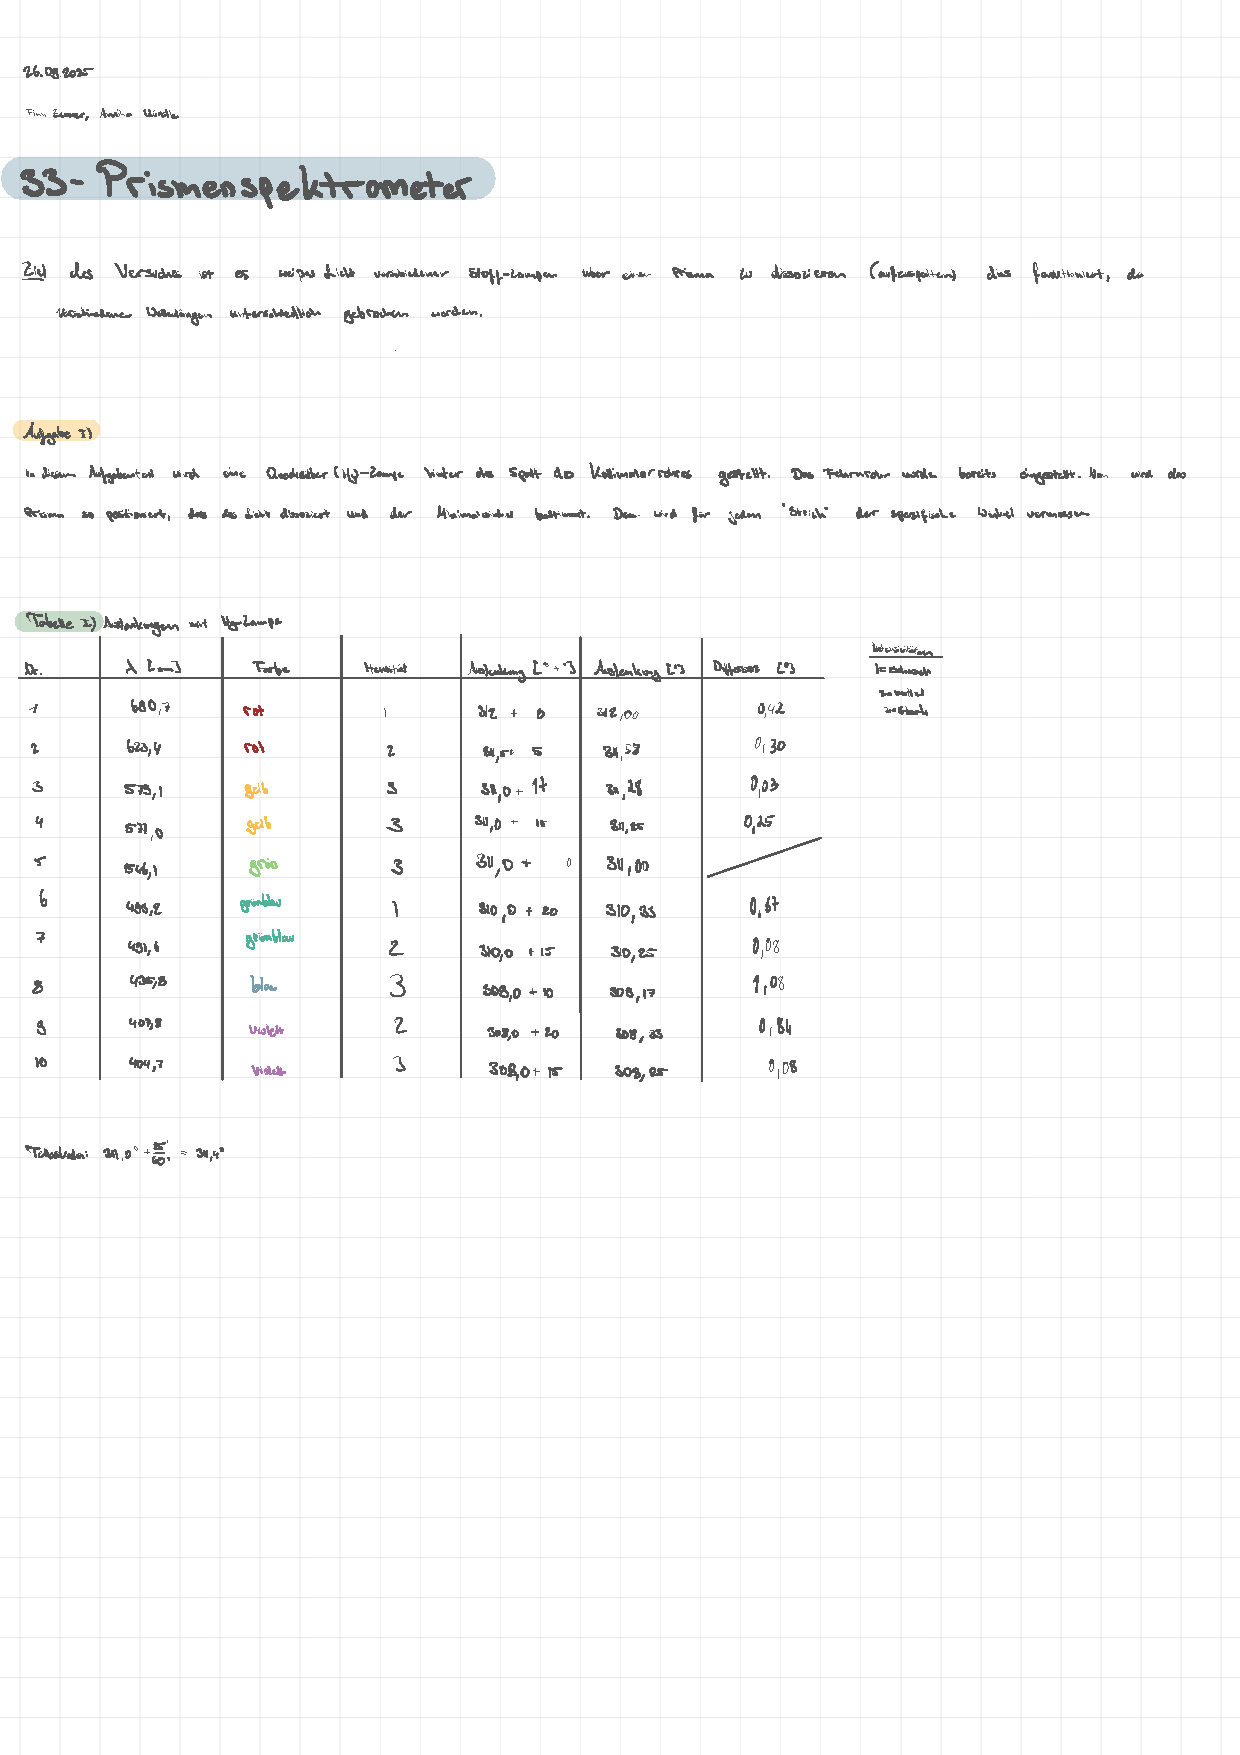
\includepdf[
  pages=-,               
  pagecommand={\thispagestyle{empty}} 
]{Protokolle/\versuchsnummer/Chapter/Messprotokoll.pdf}



\addcontentsline{lot}{table}{\protect\numberline{\thechapter.1} Schwingdauer mit Messung bei der Maximalauslenkung der Feder}
\addcontentsline{lot}{table}{\protect\numberline{\thechapter.2} Schwingdauer mit Messung durch den Nulldurchgang der Feder}
\addcontentsline{lot}{table}{\protect\numberline{\thechapter.3} Messung der Federkonstante via verschiedener Massen}
\addcontentsline{lot}{table}{\protect\numberline{\thechapter.4} Messung der Erdbeschleunigung}
